\documentclass[12pt]{article}
\usepackage{fullpage}
\usepackage{hyperref}
\hypersetup{bookmarks=true,colorlinks=true,linkcolor=red,citecolor=blue,filecolor=magenta,urlcolor=cyan}
\usepackage{amsmath}
\usepackage{longtable}
\usepackage{booktabs}
\usepackage{caption}
\usepackage{graphics}
\title{Software Requirements Specification for Solar Water Heating Systems}
\author{Thulasi Jegatheesan}
\begin{document}
\maketitle
\tableofcontents
\newpage
\section{Reference Material}
\label{Sec:RefeMate}
This section records information for easy reference.
\subsection{Table of Units}
\label{Sec:TablofUnit}
The unit system used throughout is SI (Syst\`{e}me International d'Unit\'{e}s). In addition to the basic units, several derived units are also used. For each unit, the table lists the symbol, a description and the SI name.
\begin{longtable*}{l l}
\toprule
Symbol & Description
\\
\midrule
m & length (metre)
\\
kg & mass (kilogram)
\\
s & time (second)
\\
${}^{\circ}C$ & temperature (centigrade)
\\
J & energy (joule)
\\
W & power (watt)
\\
\bottomrule
\label{Table:TablofUnit}
\end{longtable*}
\subsection{Table of Symbols}
\label{Sec:TablofSymb}
The table that follows summarizes the symbols used in this document along with their units. The choice of symbols was made to be consistent with the heat transfer literature and with existing documentation for solar water heating systems. The symbols are listed in alphabetical order.
\begin{longtable*}{l l l}
\toprule
Symbol & Description & Units
\\
\midrule
$A_{C}$ & Heating coil surface area & $\text{m}^{2}$
\\
$A_{in}$ & Surface area over which heat is transferred in & $\text{m}^{2}$
\\
$A_{out}$ & Surface area over which heat is transferred out & $\text{m}^{2}$
\\
$C^{L}$ & Specific heat capacity of a liquid & $\frac{\text{J}}{(\text{kg}{}^{\circ}C)}$
\\
$C$ & Specific heat capacity & $\frac{\text{J}}{(\text{kg}{}^{\circ}C)}$
\\
$C_{W}$ & Specific heat capacity of water & $\frac{\text{J}}{(\text{kg}{}^{\circ}C)}$
\\
$D$ & Diameter of tank & m
\\
$g$ & Volumetric heat generation per unit volume & $\frac{\text{W}}{\text{m}^{3}}$
\\
$h$ & Convective heat transfer coefficient & $\frac{\text{W}}{(\text{m}^{2}{}^{\circ}C)}$
\\
$h_{C}$ & Convective heat transfer coefficient between coil and water & $\frac{\text{W}}{(\text{m}^{2}{}^{\circ}C)}$
\\
$L$ & Length of tank & m
\\
$m$ & Mass & kg
\\
$m_{W}$ & Mass of water & kg
\\
$q$ & Heat flux & $\frac{\text{W}}{\text{m}^{2}}$
\\
$q_{in}$ & Heat flux input & $\frac{\text{W}}{\text{m}^{2}}$
\\
$q_{out}$ & Heat flux output & $\frac{\text{W}}{\text{m}^{2}}$
\\
$\mathbf{q}$ & Thermal flux vector & $\frac{\text{W}}{\text{m}^{2}}$
\\
$q_{C}$ & Heat flux into the water from the coil & $\frac{\text{W}}{\text{m}^{2}}$
\\
$T$ & Temperature & ${}^{\circ}C$
\\
$T_{C}$ & Temperature of the heating coil & ${}^{\circ}C$
\\
$T_{env}$ & Temperature of the environment & ${}^{\circ}C$
\\
$t$ & Time & s
\\
$t_{final}$ & Final time & s
\\
$T_{init}$ & Initial temperature & ${}^{\circ}C$
\\
$T_{W}$ & Temperature of the water & ${}^{\circ}C$
\\
$V_{tank}$ & Volume of the cylindrical tank & $\text{m}^{3}$
\\
$V$ & Volume & $\text{m}^{3}$
\\
$V_{W}$ & Volume of water & $\text{m}^{3}$
\\
$\Delta{}T$ & Temperature difference & ${}^{\circ}C$
\\
$\rho{}$ & Density & $\frac{\text{kg}}{\text{m}^{3}}$
\\
$\rho{}_{W}$ & Density of water & $\frac{\text{kg}}{\text{m}^{3}}$
\\
$\tau{}$ & Dummy variable for integration over time & s
\\
\bottomrule
\label{Table:TablofSymb}
\end{longtable*}
\subsection{Abbreviations and Acronyms}
\label{Sec:AbbrandAcro}
\begin{longtable*}{l l}
\toprule
Symbol & Description
\\
\midrule
A & Assumption
\\
DD & Data Definition
\\
GD & General Definition
\\
GS & Goal Statement
\\
IM & Instance Model
\\
LC & Likely Change
\\
ODE & Ordinary Differential Equation
\\
PS & Physical System Description
\\
R & Requirement
\\
SRS & Software Requirements Specification
\\
SWHS & Solar Water Heating System
\\
T & Theoretical Model
\\
\bottomrule
\label{Table:AbbrandAcro}
\end{longtable*}
\section{Introduction}
\label{Sec:Intr}
Due to increasing cost, diminishing availability, and negative environmental impact of fossil fuels, there is a higher demand for renewable energy sources and energy storage technology. Solar water heating systems provide a novel way of storing energy.
The following section provides an overview of the Software Requirements Specification (SRS) for solar water heating systems. The developed program will be referred to as Solar Water Heating System (SWHS). This section explains the purpose of this document, the scope of the system, the organization of the document, and the characteristics of the intended reader.
\subsection{Purpose of Document}
\label{Sec:PurpofDocu}
The main purpose of this document is to describe the modelling of solar water heating system. The goals and theoretical models used in the SWHS code are provided, with an emphasis on explicitly identifying assumptions and unambiguous definitions. This document is intended to be used as a reference to provide ad hoc access to all information necessary to understand and verify the model. The SRS is abstract because the contents say what problem is being solved, but do not say how to solve it.
This document will be used as a starting point for subsequent development phases, including writing the design specification and the software verification and validation plan. The design document will show how the requirements are to be realized, including decisions on the numerical algorithms and programming environment. The verification and validation plan will show the steps that will be used to increase confidence in the software documentation and the implementation. Although the SRS fits in a series of documents that follow the so-called waterfall model, the actual development process is not constrained in any way. Even when the waterfall model is not followed, as Parnas and Clements point out, the most logical way to present the documentation is still to ``fake" a rational design process.
\subsection{Scope of Requirements}
\label{Sec:ScopofRequ}
The scope of the requirements includes thermal analysis of a single solar water heating tank. Given the appropriate inputs, the code for Solar Water Heating Systems is intended to predict the temperature and thermal energy histories for the water.
\subsection{Characteristics of Intended Reader}
\label{Sec:CharofInteRead}
Reviewers of this documentation should have a strong knowledge in heat transfer theory. A third or fourth year Mechanical Engineering course on this topic is recommended. The reviewers should also have an understanding of differential equations, as typically covered in first and second year Calculus courses. The users of Solar Water Heating Systems can have a lower level of expertise, as explained in Section~\ref{Sec:UserChar}.
\subsection{Organization of Document}
\label{Sec:OrgaofDocu}
The presentation follows the standard pattern of presenting goals, theories, definitions, and assumptions. For readers that would like a more bottom up approach, they can start reading the instance models in Section~\ref{Sec:InstMode} and trace back to find any additional information they require.
The goal statements are refined to the theoretical models, and the theoretical models to the instance models.
\section{General System Description}
\label{Sec:GeneSystDesc}
This section provides general information about the system, identifies the interfaces between the system and its environment, and describes the user characteristics and the system constraints.
\subsection{System Context}
\label{Sec:SystCont}
Figure~\ref{Figure::SystCont} shows the system context. A circle represents an external entity outside the software, the user in this case. A rectangle represents the software system itself (SWHS). Arrows are used to show the data flow between the section and its environment.
\begin{figure}
\begin{center}
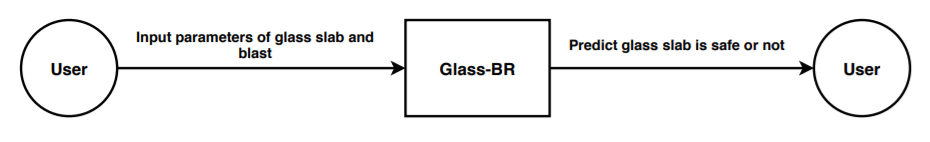
\includegraphics{SystemContextFigure.png}
\caption{Figure~\ref{Figure::SystCont}: System Context}
\label{Figure::SystCont}
\end{center}
SWHS is mostly self-contained. The only external interaction is through the user interface. The responsibilities of the user and the system are as follows:
\begin{enumerate}
\item{User Responsibilities:}
\begin{enumerate}
\item{Provide the input data to the system, ensuring no errors in the data entry}
\item{Take care that consistent units are used for input variables}
\end{enumerate}
\item{SWHS Responsibilities:}
\begin{enumerate}
\item{Detect data type mismatch, such as a string of characters instead of a floating point number}
\item{Determine if the inputs satisfy the required physical and software constraints}
\item{Calculate the required outputs}
\end{enumerate}
\end{enumerate}
\end{figure}
\subsection{User Characteristics}
\label{Sec:UserChar}
\subsection{System Constraints}
\label{Sec:SystCons}
There are no system constraints.
\section{Specific System Description}
\label{Sec:SpecSystDesc}
This section first presents the problem description, which gives a high-level view of the problem to be solved. This is followed by the solution characteristics specifications, which presents the assumptions, theories, definitions and finally the instance model (ODE) that models the solar water heating tank.
\subsection{Problem Description}
\label{Sec:ProbDesc}
SWHS is a computer program developed to investigate the heating of water in a solar water heating tank.
\subsubsection{Terminology and Definitions}
\label{Sec:TermandDefi}
This subsection provides a list of terms that are used in the subsequent sections and their meaning, with the purpose of reducing ambiguity and making it easier to correctly understand the requirements:
\begin{enumerate}
\item{Heat flux: the rate of heat energy transfer per unit area}
\item{Specific heat: heat capacity per unit mass}
\end{enumerate}
\subsubsection{Physical System Description}
\label{Sec:PhysSystDesc}
The physical system of SWHS, as shown in Figure~\ref{Figure:Solawateheattankwithheatfluxfromcoilof}, includes the following elements:
\begin{itemize}
\item[PS1:]Tank containing water
\item[PS2:]Heating coil at bottom of tank. ($q_{C}$ represents the heat flux into the water from the coil.)
\end{itemize}
\begin{figure}
\begin{center}
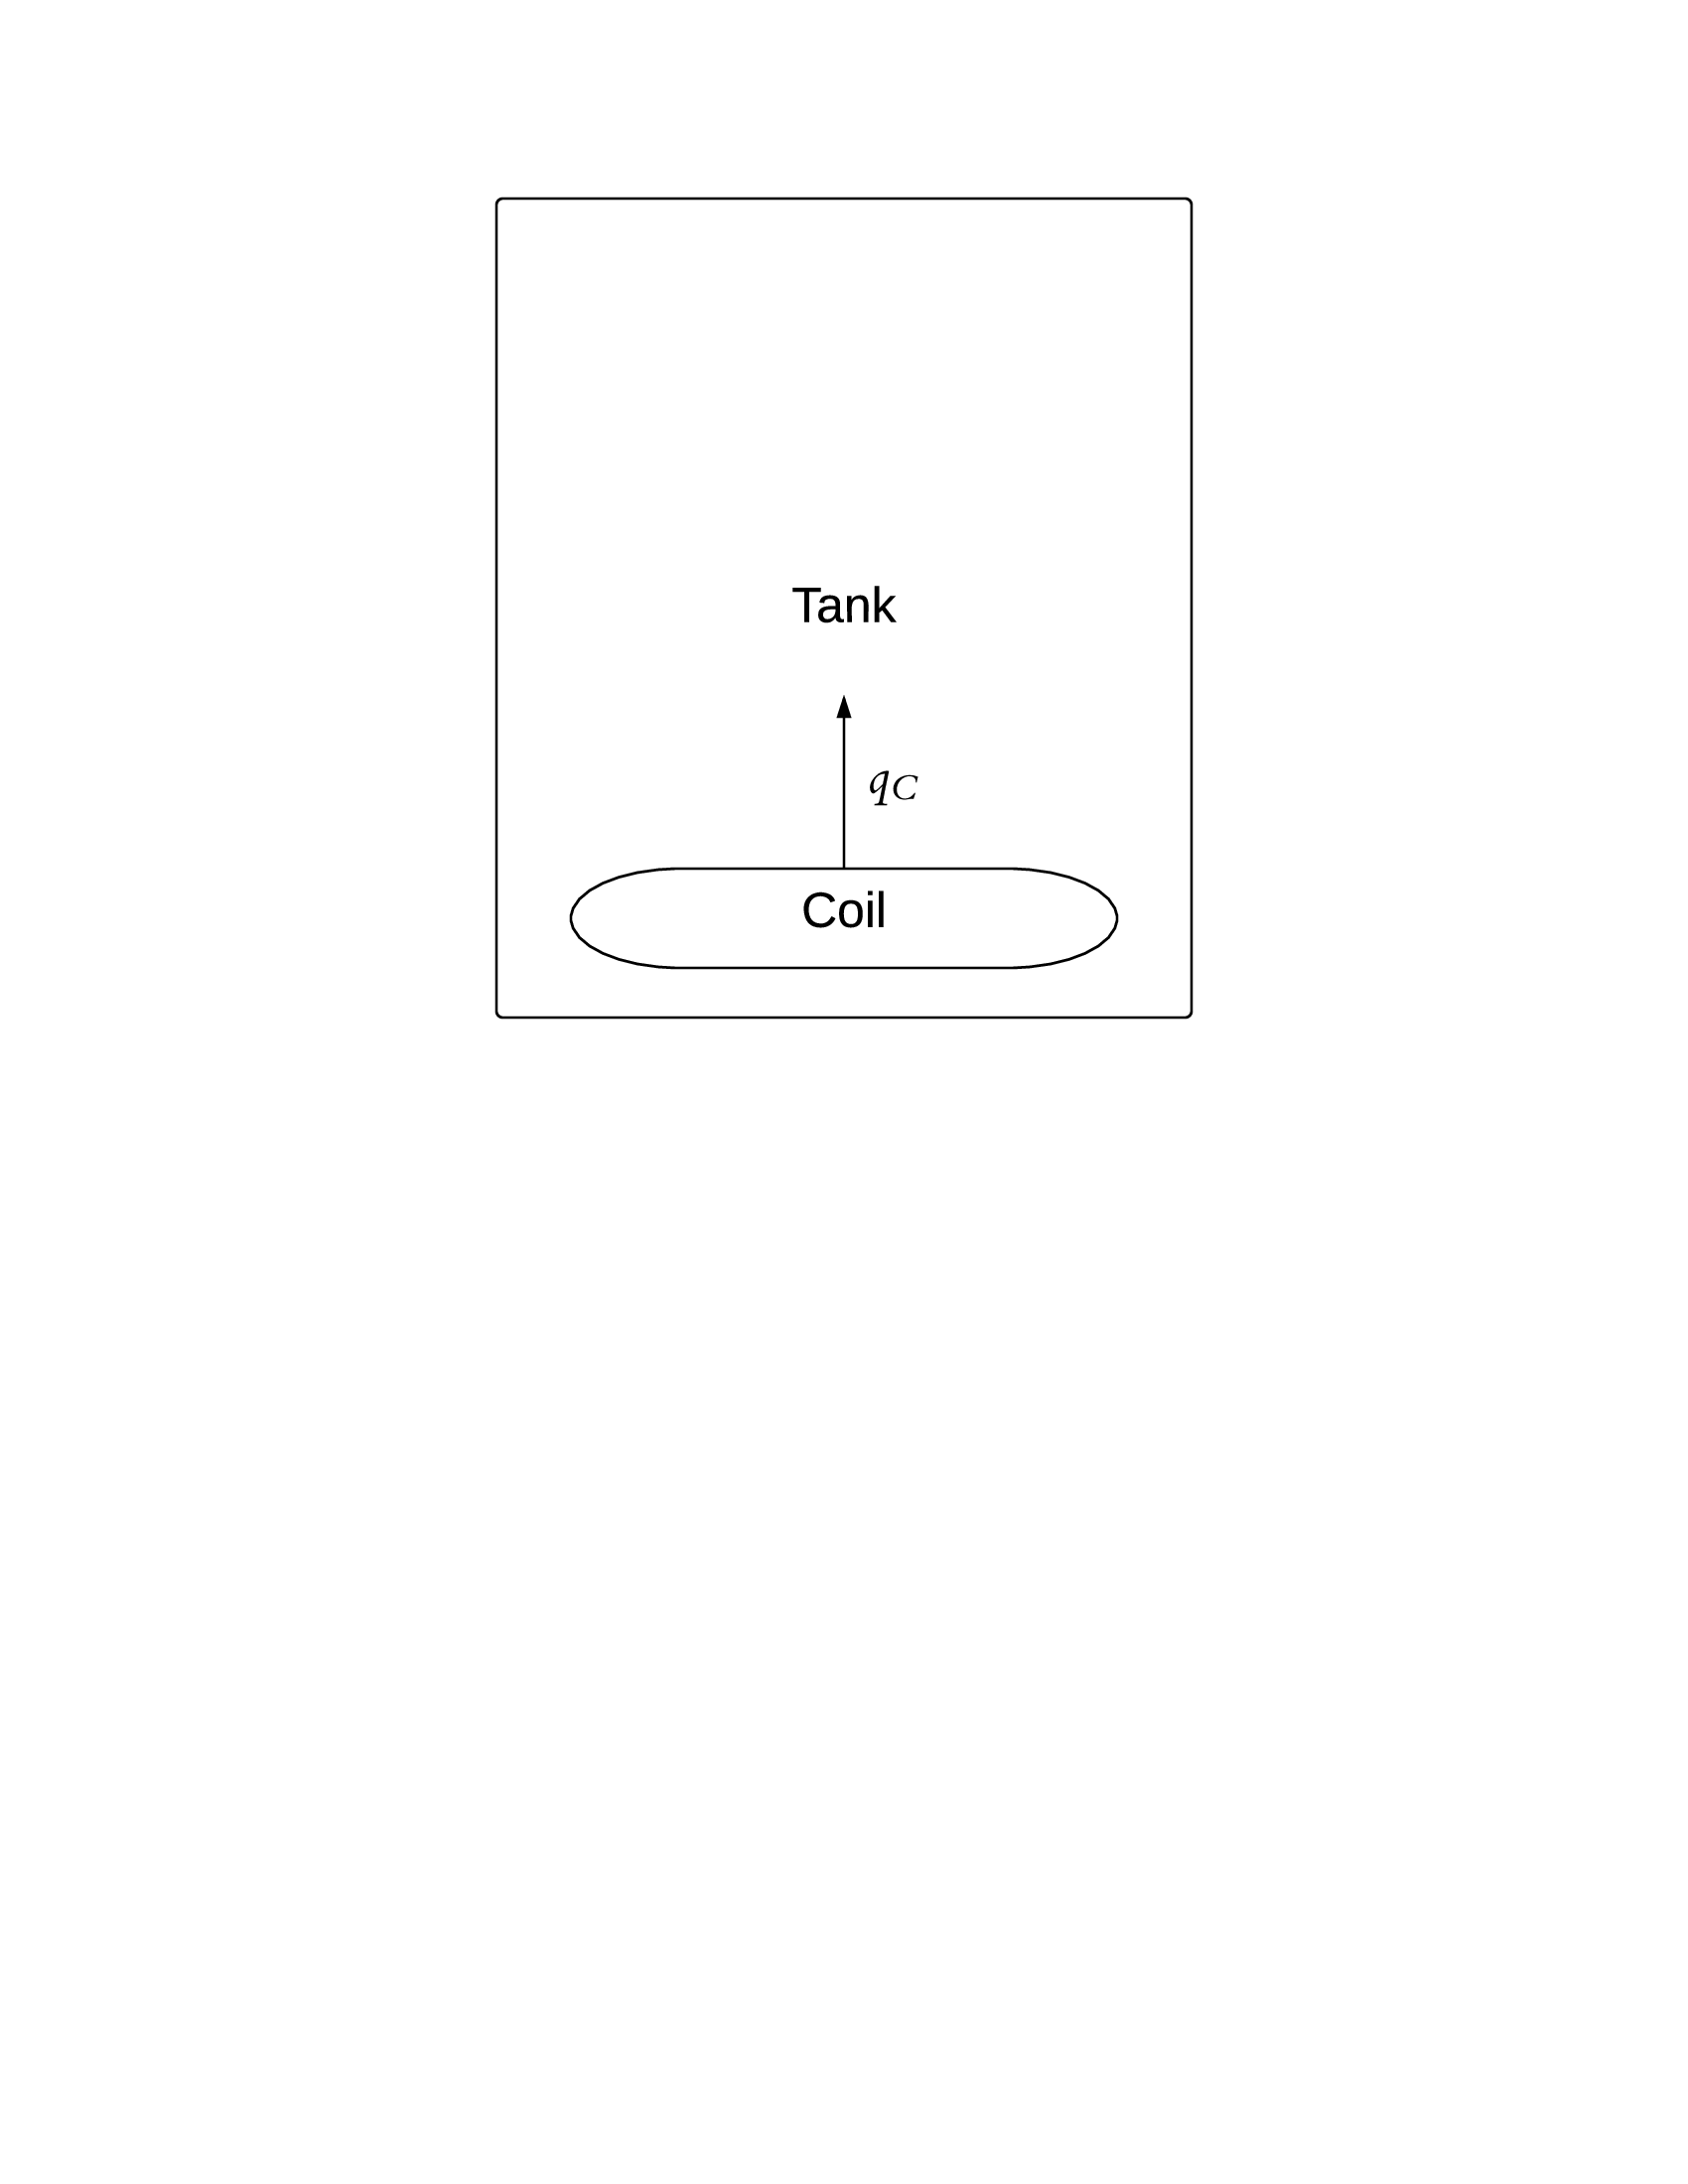
\includegraphics{TankWaterOnly.png}
\caption{Solar water heating tank, with heat flux from heating coil of $q_{C}$}
\label{Figure:Solawateheattankwithheatfluxfromcoilof}
\end{center}
\end{figure}
\subsubsection{Goal Statements}
\label{Sec:GoalStat}
Given the temperature of the heating coil, initial temperature of the water, and material properties, the goal statement is
\begin{itemize}
\item[GS1:]predict the temperature of the water over time
\end{itemize}
\subsection{Solution Characteristics Specifications}
\label{Sec:SoluCharSpec}
The instance models that govern SWHS are presented in Section~\ref{Sec:InstMode}. The information to understand the meaning of the instance models and their derivation is also presented, so that the instance models can be verified.
\subsubsection{Assumptions}
\label{Sec:Assu}
This section simplifies the original problem and helps in developing the theoretical model by filling in the missing information for the physical system. The numbers given in the square brackets refer to the Theoretical Models [Section~\ref{Sec:TheoMode}], General Definitions [Section~\ref{Sec:GeneDefi}], Data Definitions [Section~\ref{Sec:DataDefi}], Instance Models [Section~\ref{Sec:InstMode}], or Likely Changes [Section~\ref{Sec:LikeChan}], in which the respective assumption is used.
\begin{itemize}
\item[A1:]The only form of energy that is relevant for this problem is thermal energy. All other forms of energy, such as mechanical energy, are assumed to be negligible [\hyperref[T:t1ConsThermE]{Definition~T:t1ConsThermE}].
\item[A2:]All heat transfer coefficients are constant over time [GD1].
\item[A3:]The water in the tank is fully mixed, so the temperature of the water is the same throughout the entire tank [GD2].
\item[A4:]The density of water has no spatial variation; that is, it is constant over their entire volume [GD2].
\item[A5:]The specific heat capacity of water has no spatial variation; that is, it is constant over its entire volume [GD2].
\item[A6:]Newton's law of convective cooling applies between the heating coil and the water [\hyperref[DD:ht.flux.C]{Definition~DD:ht.flux.C}].
\item[A7:]The temperature of the heating coil is constant over time [\hyperref[DD:ht.flux.C]{Definition~DD:ht.flux.C}, LC1].
\item[A8:]The temperature of the heating coil does not vary along its length [\hyperref[DD:ht.flux.C]{Definition~DD:ht.flux.C}, LC2].
\item[A9:]The model only accounts for charging of the tank, not discharging. The temperature of the water can only increase, or remain constant; it cannot decrease. This implies that the initial temperature (A12) is less than (or equal) to the temperature of the heating coil [IM1, LC3].
\item[A10:]The operating temperature range of the system is such that the water is always in liquid form. That is, the temperature will not drop below the melting point temperature of water, or rise above its boiling point temperature [IM1].
\item[A11:]The tank is perfectly insulated so that there is no heat loss from the tank [IM1, LC4].
\item[A12:]No internal heat is generated by the water; therefore, the volumetric heat generation per unit volume is zero [IM1].
\end{itemize}
\subsubsection{Theoretical Models}
\label{Sec:TheoMode}
This section focuses on the general equations and laws that SWHS is based on.
~\newline
\noindent \begin{minipage}{\textwidth}
\begin{tabular}{p{0.2\textwidth} p{0.73\textwidth}}
\toprule \textbf{Refname} & \textbf{T:t1ConsThermE}
\phantomsection 
\label{T:t1ConsThermE}
\\ \midrule \\
Label & Conservation of thermal energy
\\ \midrule \\
Equation & $-\nabla{}\cdot{}\mathbf{q}+g=\rho{}C\frac{\partial{}T}{\partial{}t}$
\\ \midrule \\
Description & This equation gives the conservation of energy for time varying heat transfer in a material of specific heat capacity $C$ and density $\rho{}$, where $\mathbf{q}$ is the thermal flux vector, $g$ is the volumetric heat generation, $T$ is the temperature, $t$ is time, and $\nabla{}$ is the gradient operator. For this equation to apply, other forms of energy, such as mechanical energy, are assumed to be negligible in the.
\\ \bottomrule \end{tabular}
\end{minipage}\\
\subsubsection{General Definitions}
\label{Sec:GeneDefi}
This section collects the laws and equations that will be used in deriving the data definitions, which in turn are used to build the instance models.
~\newline
\noindent \begin{minipage}{\textwidth}
\begin{tabular}{p{0.2\textwidth} p{0.73\textwidth}}
\toprule \textbf{Refname} & \textbf{T:nwtnCooling}
\phantomsection 
\label{T:nwtnCooling}
\\ \midrule \\
Label & Newton's law of cooling
\\ \midrule \\
Equation & $\mathbf{q}\left(t\right)=h\Delta{}T\left(t\right)$
\\ \midrule \\
Description & Newton's law of cooling describes convective cooling from a surface. The law is stated as: the rate of heat loss from a body is proportional to the difference in temperatures between the body and its surroundings. Add Description.
\\ \bottomrule \end{tabular}
\end{minipage}\\
~\newline
\noindent \begin{minipage}{\textwidth}
\begin{tabular}{p{0.2\textwidth} p{0.73\textwidth}}
\toprule \textbf{Refname} & \textbf{T:rocTempSimp}
\phantomsection 
\label{T:rocTempSimp}
\\ \midrule \\
Label & Simplified rate of change of temperature
\\ \midrule \\
Equation & $mC\frac{dT}{dt}=q_{in}A_{in}-q_{out}A_{out}+gV$
\\ \midrule \\
Description & Add Description
\\ \bottomrule \end{tabular}
\end{minipage}\\
Detailed derivation of simplified rate of change of temperature:
Integrating \hyperref[T:t1ConsThermE]{Definition~T:t1ConsThermE} over a volume ($V$), we have:
\begin{equation}
\left(-\int_{V}{\nabla{}\cdot{}\mathbf{q}dV}\right)+\int_{V}{gdV}=\int_{V}{\rho{}C\frac{\partial{}T}{\partial{}t}dV}
\end{equation}
Applying Gauss's Divergence Theorem to the first term over the surface $S$ of the volume, with $\mathbf{q}$ as the thermal flux vector for the surface and $\mathbf{\hat{n}}$ as a unit outward normal vector for a surface:
\begin{equation}
\left(-\int_{S}{\mathbf{q}\cdot{}\mathbf{\hat{n}}dS}\right)+\int_{V}{gdV}=\int_{V}{\rho{}C\frac{\partial{}T}{\partial{}t}dV}
\end{equation}
We consider an arbitrary volume. The volumetric heat generation per unit volume is assumed constant. Then (1) can be written as:
\begin{equation}
q_{in}A_{in}-q_{out}A_{out}+gV=\int_{V}{\rho{}C\frac{\partial{}T}{\partial{}t}dV}
\end{equation}
Where $q_{in}$, $q_{out}$, $A_{in}$, and $A_{out}$ are explained in GD2. Assuming $\rho{}$, $C$ and $T$ are constant over the volume, which is true in our case by Assumptions (A3), (A4), and (A5), we have:
\begin{equation}
\rho{}CV\frac{dT}{dt}=q_{in}A_{in}-q_{out}A_{out}+gV
\end{equation}
Using the fact that $\rho{}$=$m$/$V$, (2) can be written as:
\begin{equation}
mC\frac{dT}{dt}=q_{in}A_{in}-q_{out}A_{out}+gV
\end{equation}
\subsubsection{Data Definitions}
\label{Sec:DataDefi}
This section collects and defines all the data needed to build the instance models. The dimension of each quantity is also given.
~\newline
\noindent \begin{minipage}{\textwidth}
\begin{tabular}{p{0.2\textwidth} p{0.73\textwidth}}
\toprule \textbf{Refname} & \textbf{DD:ht.flux.C}
\phantomsection 
\label{DD:ht.flux.C}
\\ \midrule \\
Label & $q_{C}$
\\ \midrule \\
Units & $\frac{\text{W}}{\text{m}^{2}}$
\\ \midrule \\
Equation & $q_{C}$ = $h_{C}\left(T_{C}-T_{W}\left(t\right)\right)$
\\ \midrule \\
Description & $q_{C}$ is the heat flux into the water from the coil\newline$h_{C}$ is the convective heat transfer coefficient between coil and water\newline$T_{C}$ is the temperature of the heating coil\newline$T_{W}$ is the temperature of the water\newline$t$ is the time
\\ \bottomrule \end{tabular}
\end{minipage}\\
\subsubsection{Instance Models}
\label{Sec:InstMode}
This section transforms the problem defined in Section~\ref{Sec:ProbDesc} into one which is expressed in mathematical terms. It uses concrete symbols defined in Section~\ref{Sec:DataDefi} to replace the abstract symbols in the models identified in Section~\ref{Sec:TheoMode} and Section~\ref{Sec:GeneDefi}.
~\newline
\noindent \begin{minipage}{\textwidth}
\begin{tabular}{p{0.2\textwidth} p{0.73\textwidth}}
\toprule \textbf{Refname} & \textbf{T:eBalanceOnWtr}
\phantomsection 
\label{T:eBalanceOnWtr}
\\ \midrule \\
Label & Energy balance on water to find the temperature of the water
\\ \midrule \\
Equation & $\frac{dT_{W}}{dt}=\frac{1}{\tau{}_{W}}\left(T_{C}-T_{W}\left(t\right)+\eta{}\left(T_{P}\left(t\right)-T_{W}\left(t\right)\right)\right)$
\\ \midrule \\
Description & $T_{W}$ is the temperature of the water (${}^{\circ}C$). $T_{P}$ is the temperature of the phase change material (${}^{\circ}C$). $T_{C}$ is the temperature of the heating coil (${}^{\circ}C$). $\tau{}_{W}=\frac{m_{W}C_{W}}{h_{C}A_{C}}$ is a constant (s). $\eta{}=\frac{h_{P}A_{P}}{h_{C}A_{C}}$ is a constant (dimensionless). The above equation applies as long as the water is in liquid form, $0<T_{W}<100$ (${}^{\circ}C$) where 0 (${}^{\circ}C$) and 100 (${}^{\circ}C$) are the melting and boiling point temperatures of water, respectively (A14, A19).
\\ \bottomrule \end{tabular}
\end{minipage}\\
Derivation of the energy balance on water:
To find the rate of change of $T_{W}$, we look at the energy balance on water. The volume being considered is the volume of water $V_{W}$, which has mass $m_{W}$ and specific heat capacity of water, $C_{W}$. Heat transfer occurs in the water from the coil as $q_{C}$, over area $A_{C}$. No heat transfer occurs to the outside of the tank, since it has been assumed to be perfectly insulated (A11). Assuming no volumetric heat generation per unit volume (A12), $g=0$. Therefore, the equation for GD2 can be written as:
\begin{equation}
m_{W}C_{W}\frac{dT_{W}}{dt}=q_{C}A_{C}
\end{equation}
Using \hyperref[DD:ht.flux.C]{Definition~DD:ht.flux.C}, this can be written as:
\begin{equation}
m_{W}C_{W}\frac{dT_{W}}{dt}=h_{C}A_{C}\left(T_{C}-T_{W}\right)
\end{equation}
Dividing (3) by $m_{W}$$C_{W}$, we obtain:
\begin{equation}
\frac{dT_{W}}{dt}=\frac{h_{C}A_{C}}{m_{W}C_{W}}\left(T_{C}-T_{W}\right)
\end{equation}
Setting $\tau{}_{W}$=$m_{W}$$C_{W}$/$h_{C}$$A_{C}$, Equation (4) can be written in its final form as:
\begin{equation}
\frac{dT_{W}}{dt}=\frac{1}{\tau{}_{W}}\left(T_{C}-T_{W}\right)
\end{equation}
~\newline
\noindent \begin{minipage}{\textwidth}
\begin{tabular}{p{0.2\textwidth} p{0.73\textwidth}}
\toprule \textbf{Refname} & \textbf{T:heatEInWtr}
\phantomsection 
\label{T:heatEInWtr}
\\ \midrule \\
Label & Heat energy in the water
\\ \midrule \\
Equation & $0=0$
\\ \midrule \\
Description & The above equation is derived using T2. $E_{W}$ is the change in thermal energy of the liquid water relative to the energy at the initial temperature ($T_{init}$) (J). $C_{W}$ is the specific heat capacity of liquid water ($\frac{\text{J}}{(\text{kg}{}^{\circ}C)}$) and $m_{W}$ is the mass of the water (kg). The change in temperature is the difference between the temperature at time $t$ (s), $T_{W}$ and the initial temperature, $T_{init}$ (${}^{\circ}C$). This equation applies as long as $0<T_{W}<0$${}^{\circ}C$ (A14, A19).
\\ \bottomrule \end{tabular}
\end{minipage}\\
\subsubsection{Data Constraints}
\label{Sec:DataCons}
Table~\ref{Table:Tabl1:InpuVari} and Table~\ref{Table:Tabl2:OutpVari} show the data constraints on the input and output variables, respectively. The column for physical constraints gives the physical limitations on the range of values that can be taken by the variable. The constraints are conservative, to give the user of the model the flexibility to experiment with unusual situations. The column of typical values is intended to provide a feel for a common scenario.
\begin{longtable}{l l l}
\toprule
Var & Physical Constraints & Software Constraints & Typical Value & Uncertainty
\\
\midrule
$L$ & $L>0$ & $L_{min}\leq{}L\leq{}L_{max}$ & $1.5$ m & 0.1
\\
$D$ & $D>0$ & $\frac{D}{L_{max}}\leq{}\frac{D}{L}\leq{}\frac{D}{L_{min}}$ & $0.412$ m & 0.1
\\
$A_{C}$ & $A_{C}>0$ (*) & $A_{C}\leq{}A_{C}^{max}$ & $0.12$ $\text{m}^{2}$ & 0.1
\\
$T_{C}$ & $0<T_{C}<100$ (+) &  & $50$ ${}^{\circ}C$ & 0.1
\\
$\rho{}_{W}$ & $\rho{}_{W}>0$ & $\rho{}_{W}^{min}<\rho{}_{W}\leq{}\rho{}_{W}^{max}$ & $1000$ $\frac{\text{kg}}{\text{m}^{3}}$ & 0.1
\\
$C_{W}$ & $C_{W}>0$ & $C_{W}^{min}<C_{W}<C_{W}^{max}$ & $4186$ $\frac{\text{J}}{(\text{kg}{}^{\circ}C)}$ & 0.1
\\
$h_{C}$ & $h_{C}>0$ & $h_{C}^{min}\leq{}h_{C}\leq{}h_{C}^{max}$ & $1000$ $\frac{\text{W}}{(\text{m}^{2}{}^{\circ}C)}$ & 0.1
\\
$T_{init}$ & $0<T_{init}<T_{melt}$ (+) &  & $40$ ${}^{\circ}C$ & 0.1
\\
$t_{final}$ & $t_{final}>0$ & $t_{final}<t_{final}^{max}$ (**) & $50000$ s & 0.1
\\
\bottomrule
\caption{Table 1: Input Variables}
\label{Table:Tabl1:InpuVari}
\end{longtable}
\begin{longtable}{l l l}
\toprule
Var & Physical Constraints & Software Constraints & Typical Value & Uncertainty
\\
\midrule
\bottomrule
\caption{Table 2: Output Variables}
\label{Table:Tabl2:OutpVari}
\end{longtable}
\section{Requirements}
\label{Sec:Requ}
This section provides the functional requirements, the business tasks that the software is expected to complete, and the non-functional requirements, the qualities that the software is expected to exhibit.
\subsection{Functional Requirements}
\label{Sec:FuncRequ}
\begin{itemize}
\item[R1:]Input the following quantities, which define the tank parameters, material properties and initial conditions:
\end{itemize}
\begin{longtable*}{l l l}
\toprule
Symbol & Unit & Description
\\
\midrule
$L$ & m & length of tank
\\
$D$ & m & diameter of tank
\\
$A_{C}$ & $\text{m}^{2}$ & heating coil surface area
\\
$T_{C}$ & ${}^{\circ}C$ & temperature of the heating coil
\\
$\rho{}_{W}$ & $\frac{\text{kg}}{\text{m}^{3}}$ & density of water
\\
$C_{W}$ & $\frac{\text{J}}{(\text{kg}{}^{\circ}C)}$ & specific heat capacity of water
\\
$H_{f}$ & $\frac{\text{J}}{\text{kg}}$ & specific latent heat of fusion
\\
$T_{init}$ & ${}^{\circ}C$ & initial temperature
\\
$t_{final}$ & s & final time
\\
\bottomrule
\label{Table:InpuVariRequ}
\end{longtable*}
\begin{itemize}
\item[R2:]Use the inputs in R1 to find the mass needed for IM1 to IM4, as follows, where $V_{W}$ is the volume of water and $V_{tank}$ is the volume of the cylindrical tank.
\end{itemize}
\begin{equation}
m_{W}=V_{W}\rho{}_{W}=\frac{D}{2}L\rho{}_{W}
\end{equation}
\begin{itemize}
\item[R3:]Verify that the inputs satisfy the required physical constraint shown in Table~\ref{Table:Tabl1:InpuVari}.
\end{itemize}
\begin{itemize}
\item[R4:]Outputs and inputs quantities and derived quantities in the following list: the quantities from R1, the mass from R2 and $\tau{}_{W}$ (from IM1).
\end{itemize}
\begin{itemize}
\item[R5:]Calculate and output the temperature of the water ($T_{W}$($t$)) over the simulation time.
\end{itemize}
\subsection{Non-Functional Requirements}
\label{Sec:Non-Requ}
This problem is small in size and relatively simple, so performance is not a priority. Any reasonable implementation will be very quick and use minimal storage. Rather than performance, the non-functional requirement priorities are correctness, verifiability, understandability, reusability, and maintainability.
\section{Likely Changes}
\label{Sec:LikeChan}
\begin{itemize}
\item[LC1:]A7 - The temperature of the heating coil will change over the course of the day, depending on the energy received from the sun.
\item[LC2:]A8 - The temperature of the heating coil will actually change along its length as the water within it cools.
\item[LC3:]A9 - The model currently only accounts for charging of the tank. A more complete model would also account for discharging of the tank.
\item[LC4:]A11 - Any real tank cannot be perfectly insulated and will lose heat.
\end{itemize}
\section{Traceability Matrices and Graphs}
\label{Sec:TracMatrandGrap}
The purpose of the traceability matrices is to provide easy references on what has to be additionally modified if a certain component is changed. Every time a component is changed, the items in the column of that component that are marked with an ``X" should be modified as well. Table~\ref{Table:TracMatrShowtheConnBetwRequandInstMode} shows the dependencies of theoretical models, general definitions, data definitions, and instance models with each other. Table~\ref{Table:TracMatrShowtheConnBetwRequandInstMode} shows the dependencies of instance models, requirements, and data constraints on each other. Table~\ref{Table:TracMatrShowtheConnBetwAssuandOtheItem} shows the dependencies of theoretical models, general definitions, data definitions, instance models, and likely changes on the assumptions.
\begin{longtable}{l l l l l l l}
\toprule
 & T1 (\hyperref[T:t1ConsThermE]{Definition~T:t1ConsThermE}) & GD1 (\hyperref[T:nwtnCooling]{Definition~T:nwtnCooling}) & GD2 (\hyperref[T:rocTempSimp]{Definition~T:rocTempSimp}) & DD1 (\hyperref[DD:ht.flux.C]{Definition~DD:ht.flux.C}) & IM1 (\hyperref[T:eBalanceOnWtr]{Definition~T:eBalanceOnWtr}) & IM2 (\hyperref[T:heatEInWtr]{Definition~T:heatEInWtr})
\\
\midrule
T1 (\hyperref[T:t1ConsThermE]{Definition~T:t1ConsThermE}) &  &  &  &  &  & 
\\
GD1 (\hyperref[T:nwtnCooling]{Definition~T:nwtnCooling}) &  &  &  &  &  & 
\\
GD2 (\hyperref[T:rocTempSimp]{Definition~T:rocTempSimp}) & X &  &  &  &  & 
\\
DD1 (\hyperref[DD:ht.flux.C]{Definition~DD:ht.flux.C}) &  & X &  &  &  & 
\\
IM1 (\hyperref[T:eBalanceOnWtr]{Definition~T:eBalanceOnWtr}) &  &  & X & X &  & 
\\
IM2 (\hyperref[T:heatEInWtr]{Definition~T:heatEInWtr}) &  &  &  &  &  & 
\\
\bottomrule
\caption{Traceability Matrix Showing the Connections Between Requirements and Instance Models}
\label{Table:TracMatrShowtheConnBetwRequandInstMode}
\end{longtable}
\begin{longtable}{l l l l l l l l l l}
\toprule
 & IM1 (\hyperref[T:eBalanceOnWtr]{Definition~T:eBalanceOnWtr}) & IM2 (\hyperref[T:heatEInWtr]{Definition~T:heatEInWtr}) & Data Constraints (Table~\ref{Table:InpuDataCons}) & R1 (Section~\ref{Sec:FuncRequ}) & R2 (Section~\ref{Sec:FuncRequ}) & R3 (Section~\ref{Sec:FuncRequ}) & R4 (Section~\ref{Sec:FuncRequ}) & R5 (Section~\ref{Sec:FuncRequ}) & R6 (Section~\ref{Sec:FuncRequ})
\\
\midrule
IM1 (\hyperref[T:eBalanceOnWtr]{Definition~T:eBalanceOnWtr}) &  &  &  &  &  &  &  &  & 
\\
IM2 (\hyperref[T:heatEInWtr]{Definition~T:heatEInWtr}) &  &  &  &  &  &  &  &  & 
\\
R1 (Section~\ref{Sec:FuncRequ}) &  &  &  &  &  &  &  &  & 
\\
R2 (Section~\ref{Sec:FuncRequ}) &  &  &  & X &  &  &  &  & 
\\
R3 (Section~\ref{Sec:FuncRequ}) &  &  & X &  &  &  &  &  & 
\\
R4 (Section~\ref{Sec:FuncRequ}) &  &  &  & X & X &  &  &  & 
\\
R5 (Section~\ref{Sec:FuncRequ}) & X &  &  &  &  &  &  &  & 
\\
R6 (Section~\ref{Sec:FuncRequ}) &  & X &  &  &  &  &  &  & 
\\
\bottomrule
\caption{Traceability Matrix Showing the Connections Between Requirements and Instance Models}
\label{Table:TracMatrShowtheConnBetwRequandInstMode}
\end{longtable}
\begin{longtable}{l l l l l l l l l l l l l l l}
\toprule
 & A1 (Section~\ref{Sec:InstMode}) & A2 (Section~\ref{Sec:InstMode}) & A3 (Section~\ref{Sec:InstMode}) & A4 (Section~\ref{Sec:InstMode}) & A5 (Section~\ref{Sec:InstMode}) & A6 (Section~\ref{Sec:InstMode}) & A7 (Section~\ref{Sec:InstMode}) & A8 (Section~\ref{Sec:InstMode}) & A9 (Section~\ref{Sec:InstMode}) & A10 (Section~\ref{Sec:InstMode}) & A11 (Section~\ref{Sec:InstMode}) & A12 (Section~\ref{Sec:InstMode}) & A13 (Section~\ref{Sec:InstMode}) & A14 (Section~\ref{Sec:InstMode})
\\
\midrule
T1 (\hyperref[T:t1ConsThermE]{Definition~T:t1ConsThermE}) & X &  &  &  &  &  &  &  &  &  &  &  &  & 
\\
GD1 (\hyperref[T:nwtnCooling]{Definition~T:nwtnCooling}) &  & X &  &  &  &  &  &  &  &  &  &  &  & 
\\
GD2 (\hyperref[T:rocTempSimp]{Definition~T:rocTempSimp}) &  &  & X & X & X &  &  &  &  &  &  &  &  & 
\\
DD1 (\hyperref[DD:ht.flux.C]{Definition~DD:ht.flux.C}) &  &  &  &  &  & X & X & X &  &  &  &  &  & 
\\
IM1 (\hyperref[T:eBalanceOnWtr]{Definition~T:eBalanceOnWtr}) &  &  &  &  &  &  &  &  & X & X &  &  &  & 
\\
IM2 (\hyperref[T:heatEInWtr]{Definition~T:heatEInWtr}) &  &  &  &  &  &  &  &  &  & X &  &  &  & 
\\
LC1 (Section~\ref{Sec:LikeChan}) &  &  &  &  &  &  & X &  &  &  &  &  &  & 
\\
LC2 (Section~\ref{Sec:LikeChan}) &  &  &  &  &  &  &  & X &  &  &  &  &  & 
\\
LC3 (Section~\ref{Sec:LikeChan}) &  &  &  &  &  &  &  &  & X &  &  &  &  & 
\\
LC4 (Section~\ref{Sec:LikeChan}) &  &  &  &  &  &  &  &  &  &  & X &  &  & 
\\
\bottomrule
\caption{Traceability Matrix Showing the Connections Between Assumptions and Other Items}
\label{Table:TracMatrShowtheConnBetwAssuandOtheItem}
\end{longtable}
The purpose of the traceability graphs is also to provide easy references on what has to be additionally modified if a certain component is changed. The arrows in the graphs represent dependencies. The component at the tail of an arrow is depended on by the component at the head of that arrow. Therefore, if a component is changed, the components that it points to should also be changed. Figure~\ref{Figure:TracGrapShowtheConnBetwItemofDiffSect} shows the dependencies of theoretical models, general definitions, data definitions, instance models, likely changes, and assumptions on each other. Figure~\ref{Figure:TracGrapShowtheConnBetwRequInstModeandDataCons} shows the dependencies of instance models, requirements, and data constraints on each other.
NOTE: Building a tool to automatically generate the graphical representation of the matrix by scanning the labels and reference can be future work.
\begin{figure}
\begin{center}
\includegraphics{ATrace.png}
\caption{Traceability Graph Showing the Connections Between Items of Different Sections}
\label{Figure:TracGrapShowtheConnBetwItemofDiffSect}
\end{center}
\end{figure}
\begin{figure}
\begin{center}
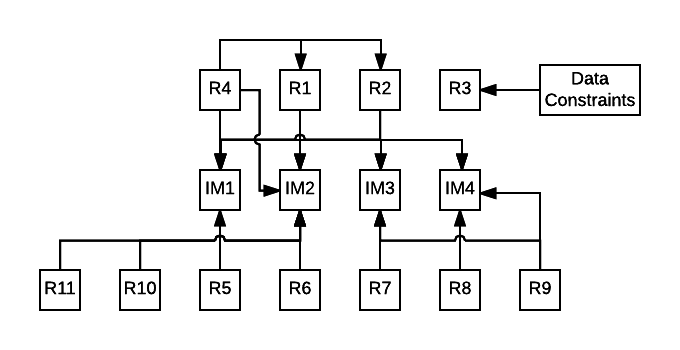
\includegraphics{RTrace.png}
\caption{Traceability Graph Showing the Connections Between Requirements, Instance Models, and Data Constraints}
\label{Figure:TracGrapShowtheConnBetwRequInstModeandDataCons}
\end{center}
\end{figure}
\section{Values Of Auxiliary Constants}
\label{Sec:ValuOfAuxiCons}
This section contains the standard values that are used for calculations in SWHS.
\begin{longtable}{l l l l}
\toprule
Symbol & Description & Value & Unit
\\
\midrule
$L_{min}$ & minimum length of tank & $\frac{1}{10}$ & m
\\
$L_{max}$ & maximum length of tank & $50$ & m
\\
$h_{min}$ & minimum convective heat transfer coefficient & $0.001$ & $\frac{\text{W}}{(\text{m}^{2}{}^{\circ}C)}$
\\
$\rho{}_{W}^{min}$ & minimum density of water & $950$ & $\frac{\text{kg}}{\text{m}^{3}}$
\\
$\rho{}_{W}^{max}$ & maximum density of water & $1000$ & $\frac{\text{kg}}{\text{m}^{3}}$
\\
$C_{W}^{min}$ & minimum specific heat capacity of water & $4170$ & $\frac{\text{J}}{(\text{kg}{}^{\circ}C)}$
\\
$C_{W}^{max}$ & maximum specific heat capacity of water & $4210$ & $\frac{\text{J}}{(\text{kg}{}^{\circ}C)}$
\\
$h_{C}^{min}$ & minimum convective heat transfer coefficient between coil and water & $10$ & $\frac{\text{W}}{(\text{m}^{2}{}^{\circ}C)}$
\\
$h_{C}^{max}$ & maximum convective heat transfer coefficient between coil and water & $10000$ & $\frac{\text{W}}{(\text{m}^{2}{}^{\circ}C)}$
\\
$t_{final}^{max}$ & maximum final time & $86400$ & s
\\
\bottomrule
\caption{Auxiliary Constants}
\label{Table:AuxiCons}
\end{longtable}
\section{References}
\label{Sec:Refe}
\begin{itemize}
\item[[1]:]F. P. Incropera, D. P. Dewitt, T. L. Bergman, and A. S. Lavine. Fundamentals of Heat and Mass Transfer. John Wiley and Sons, United States, sixth edition edition, 2007.
\item[[2]:]Nirmitha Koothoor. A document drive approach to certifying scientific computing software. Master's thesis, McMaster University, Hamilton, Ontario, Canada, 2013.
\item[[3]:]Marilyn Lightstone. Derivation of tank/pcm model. Personal Notes, 2012.
\item[[4]:]David L. Parnas and P.C. Clements. A rational design process: How and why to fake it. IEEE Transactions on Software Engineering, 12``2":251-257, February 1986.
\item[[5]:]W. Spencer Smith and Lei Lai. A new requirements template for scientific computing. In J. Ralyt\'{e}, P. Agerfalk, and N. Kraiem, editors, Proceedings of the First International Workshop on Situational Requirements Engineering Processes - Methods, Techniques and Tools to Support Situation-Specific Requirements Engineering Processes, SREP'05, pages 107-121, Paris, France, 2005. In conjunction with 13th IEEE International Requirements Engineering Conference.
\end{itemize}
\end{document}
